% !TEX root = trkjet.tex

The following sources of systematic uncertainty are considered:
the jet energy scale (JES), the jet energy resolution (JER), 
the sensitivity of the  unfolding to the prior, the UE contribution, the residual non-closure of the analysis procedure, and tracking-related uncertainties.
For each systematic variation, the \Dptr\ distributions along with their ratios and differences are re-evaluated. The difference between the varied and nominal distributions is used as an estimate of the uncertainty.

The systematic uncertainty due to the JES in \PbPb\ collisions is composed of two parts: 
a centrality-independent baseline component and a centrality-dependent component. Only the centrality-independent baseline component is used in \pp\ collisions; 
it is determined from \textit{in-situ} studies of the calorimeter
response~\cite{Aad:2011he,HIjesnote,Aaboud:2017jcu} and the relative energy scale difference between the jet reconstruction procedures in heavy-ion~\cite{HIjesnote} and \pp\ collisions~\cite{Aad:2014bia}. The centrality-dependent uncertainty reflects a modification of parton showers by the \PbPb\ environment. It is evaluated by comparing calorimeter \ptjet\ and the sum of the transverse momentum of charged particles within the jet in data and MC. The size of the centrality-dependent uncertainty on the JES reaches 0.5\% in the most central collisions. Each component that contributes to the JES uncertainty is varied separately by $\pm1$ standard deviation for each interval in \ptjet\ and the response matrix is recomputed accordingly. The data are then unfolded with the modified matrices. The resulting uncertainty from the JES increases with increasing charged-particle \pT\ at fixed \ptjet\ and decreases with increasing \ptjet, and is at the level of 2--4\%.

The uncertainty on the \Dptr\ distributions due to the JER is evaluated by repeating the unfolding procedure with modified response matrices, where an additional contribution is added to the resolution of the reconstructed \ptjet\ using a Gaussian smearing procedure. The smearing factor is evaluated using an \textit{in-situ} technique in 13~\TeV\ \pp\ data that involves studies of dijet energy balance~\cite{Aad:2012ag,JERConfNote}. An additional uncertainty is included to account for differences between the tower-based jet reconstruction and that used in analyses of 13~\TeV\ \pp\ data. The resulting uncertainty from the JER is symmetrized to account for negative variations of the JER.  The size of the resulting uncertainty on the \Dptr\ distributions due to the JER typically reaches 4--5\% for the highest charged-particle \pT\ intervals and decreases to 2--3\% with decreasing charged-particle \pT\ at fixed \ptjet.


The uncertainties related to track reconstruction and selection originate from several sources.
Uncertainties related to the material description in simulation and the track transverse 
momentum resolution are obtained from studies in data and simulation described in Ref.~\cite{ATL-PHYS-PUB-2015-051}.
The sensitivity of the tracking efficiency to the description of the 
inactive material in the MC samples is evaluated by varying the material description.
This resulting uncertainty in the track reconstruction efficiency is between
0.5\% and 2\% in the track \pT\ range used in the analysis. 
The systematic uncertainty on the fakes and secondaries is 30\% in both collision systems~\cite{ATL-PHYS-PUB-2015-051}.  The contamination of fake tracks is less than 2\% and the resulting uncertainty in the \Dptr\ distributions is at most 5\%.
An additional uncertainty takes into account a possible residual misalignment of the tracking detectors
in \pp\ and \PbPb\ data-taking. The alignment in these datasets is checked \textit{in-situ} with $Z\rightarrow \mu^{+}\mu^{-}$ events, and the track-\pT\-dependent uncertainty arises from the finite size of this sample. The resulting uncertainties in
the \Dptr\ distributions are typically less than 0.1\%. An additional  uncertainty in the tracking efficiency due to the high local track density in the core of jets is 0.4\%~\cite{ATL-PHYS-PUB-2016-007} for all \ptjet\ ranges in this analysis. The uncertainty due to the track selection is evaluated by repeating the analysis with an additional requirement on the significance of the distance of closest approach of the track to the primary vertex. This uncertainty affects 
the track reconstruction efficiencies, track momentum resolution, and rate of fake tracks. The resulting uncertainty typically varies between 1--2\%.
Finally, the track-to-particle association requirements are varied. This variation affects the track reconstruction efficiency, track momentum resolution, and rate of fake tracks. The resulting systematic uncertainty is $\leq~0.1 \%$ on the \Dptr\ distributions. All track-related systematic uncertainties are added in quadrature and presented as the total tracking uncertainty. 

The systematic uncertainty associated with the UE subtraction has two components: limited statistics of charged particles associated with a jet without a corresponding generator particle in the \pbpb\ MC, and a comparison to an alternative UE estimation done using the cone method. The cone method uses jet triggered events to estimate the background and is adapted from \cite{Aaboud:2018hpb, Aaboud:2017bzv}. A regular grid of 9 cones of size $R = 0.8$ is used to cover the inner detector region. Cones are excluded if they are within an angular distance of 1.6 to a reconstructed jet with $\ptjet > 90$ GeV or if they contain a charged particle with \mbox{$\pt > 10$ GeV}. This exclusion reduces biases from any hard processes. The resulting UE charged particle yields $\fd \nchUE^{\mathrm{Cone}}/ \fd \pTch$ are evaluated over the \mbox{1--10 GeV} range as a function of \pttrk, \ptjet, centrality, and \rvar, and are subsequently averaged over all cones. The UE uncertainty on the \Dptr\ distributions is approximately 40\% at the largest angular distances from the jet axis and rapidly decreases with increasing charged-particle \pT\ and decreasing distance. This is the dominant source of the systematic uncertainty at low charged-particle \pt\ and large \rvar. In particular, the component from the limited statistics dominates in the most central collisions, while the component from the alternative estimation method dominates elsewhere.


The systematic uncertainty on the unfolding procedure is estimated by generating the response matrices from the MC distributions without any re-weighting to match shapes in data. Conservatively, the difference between the nominal \Dptr\ distribution and \Dptr\ unfolded with the un-reweighted response matrices is taken as the systematic uncertainty, and is at the level of 5--7\%.

Conservatively, an additional uncertainty to account for possible residual limitations in the analysis procedure is assigned by evaluating the non-closure of the unfolded distributions in simulations. This is typically at the level of 3-4\% and is described in Section~\ref{sec:analysis}.

The correlations between the various systematic components are considered in evaluating the \RDptr\ and $\Delta\Dptr$ distributions. The unfolding and non-closure uncertainties are taken to be uncorrelated between \pp\ and \pbpb\ collisions, while all others are taken to be correlated. For these, the \RDptr\ and $\Delta\Dptr$ distributions are re-evaluated by applying the variation to both collision systems; the resulting variations of the ratios from their central values are used as the correlated systematic uncertainty. 

Examples of systematic uncertainties in the \Dptr\ distributions for jets in the 126--158~\GeV\ \ptjet\ 
range measured in \pp\ and \pbpb\ collision systems are shown in Figure~\ref{fig:Systematics_Dpt}. The uncertainties on the \RDptr\ distributions are shown in Figure~\ref{fig:Systematics_RDpT}. It can be seen that the dominant systematic uncertainty on the \pbpb\ and the \RDptr\ distributions is from the underlying event estimation. While it is less than 5\% for $r < 0.3$ from the jet axis, it is approximately 40\% for charged particles with $\pt = 1$ GeV at $r = 0.8$ from the jet axis. The uncertainties in the \pp\ system are smaller, with the dominant systematic uncertainty coming from the tracking. This uncertainty is approximately 10\%  for $r < 0.1$ and decreases to less than 5\% at larger distances.

\begin{figure}
\centerline{
\begin{tabular}{cc}
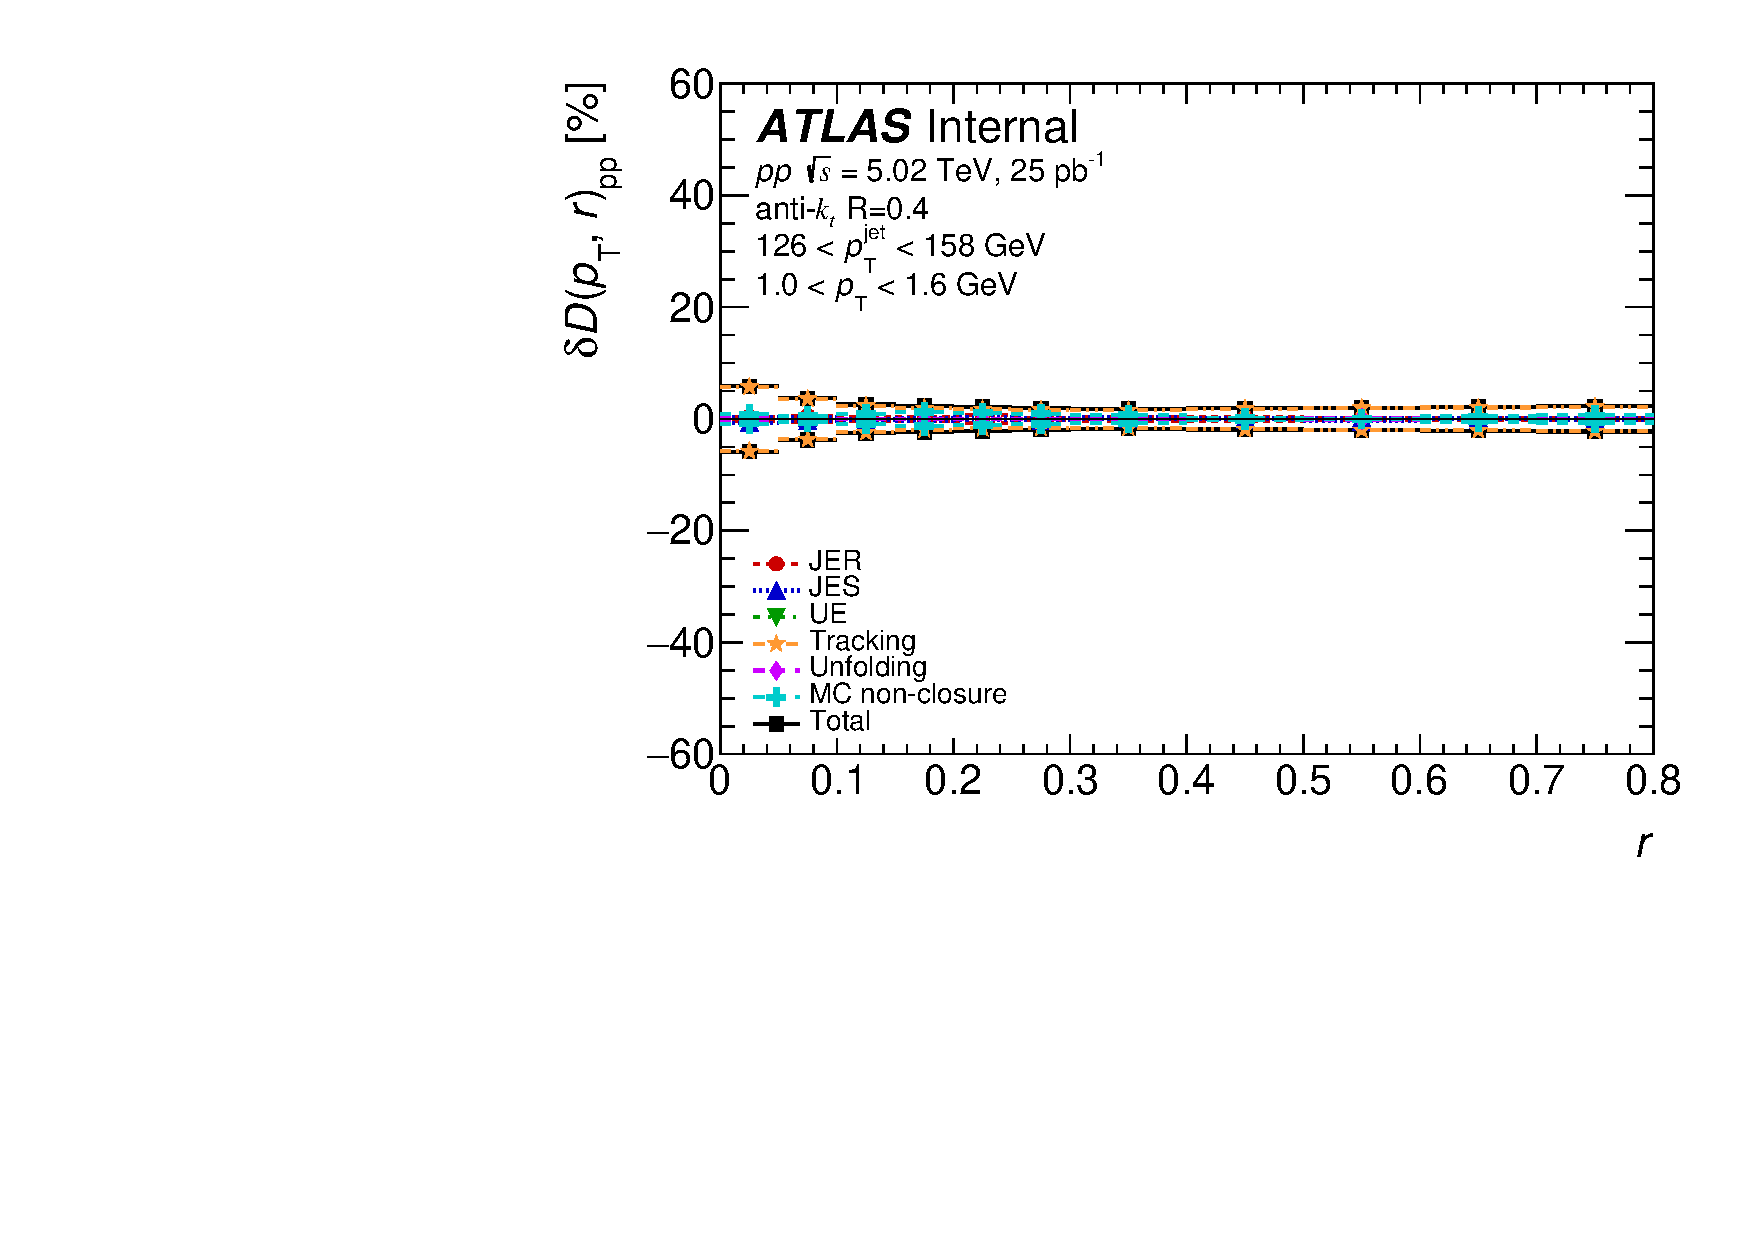
\includegraphics[width=0.53\textwidth]{figures/systematics/ChPS_dR_sys_pp_error_trk2_jet7_cent6} &
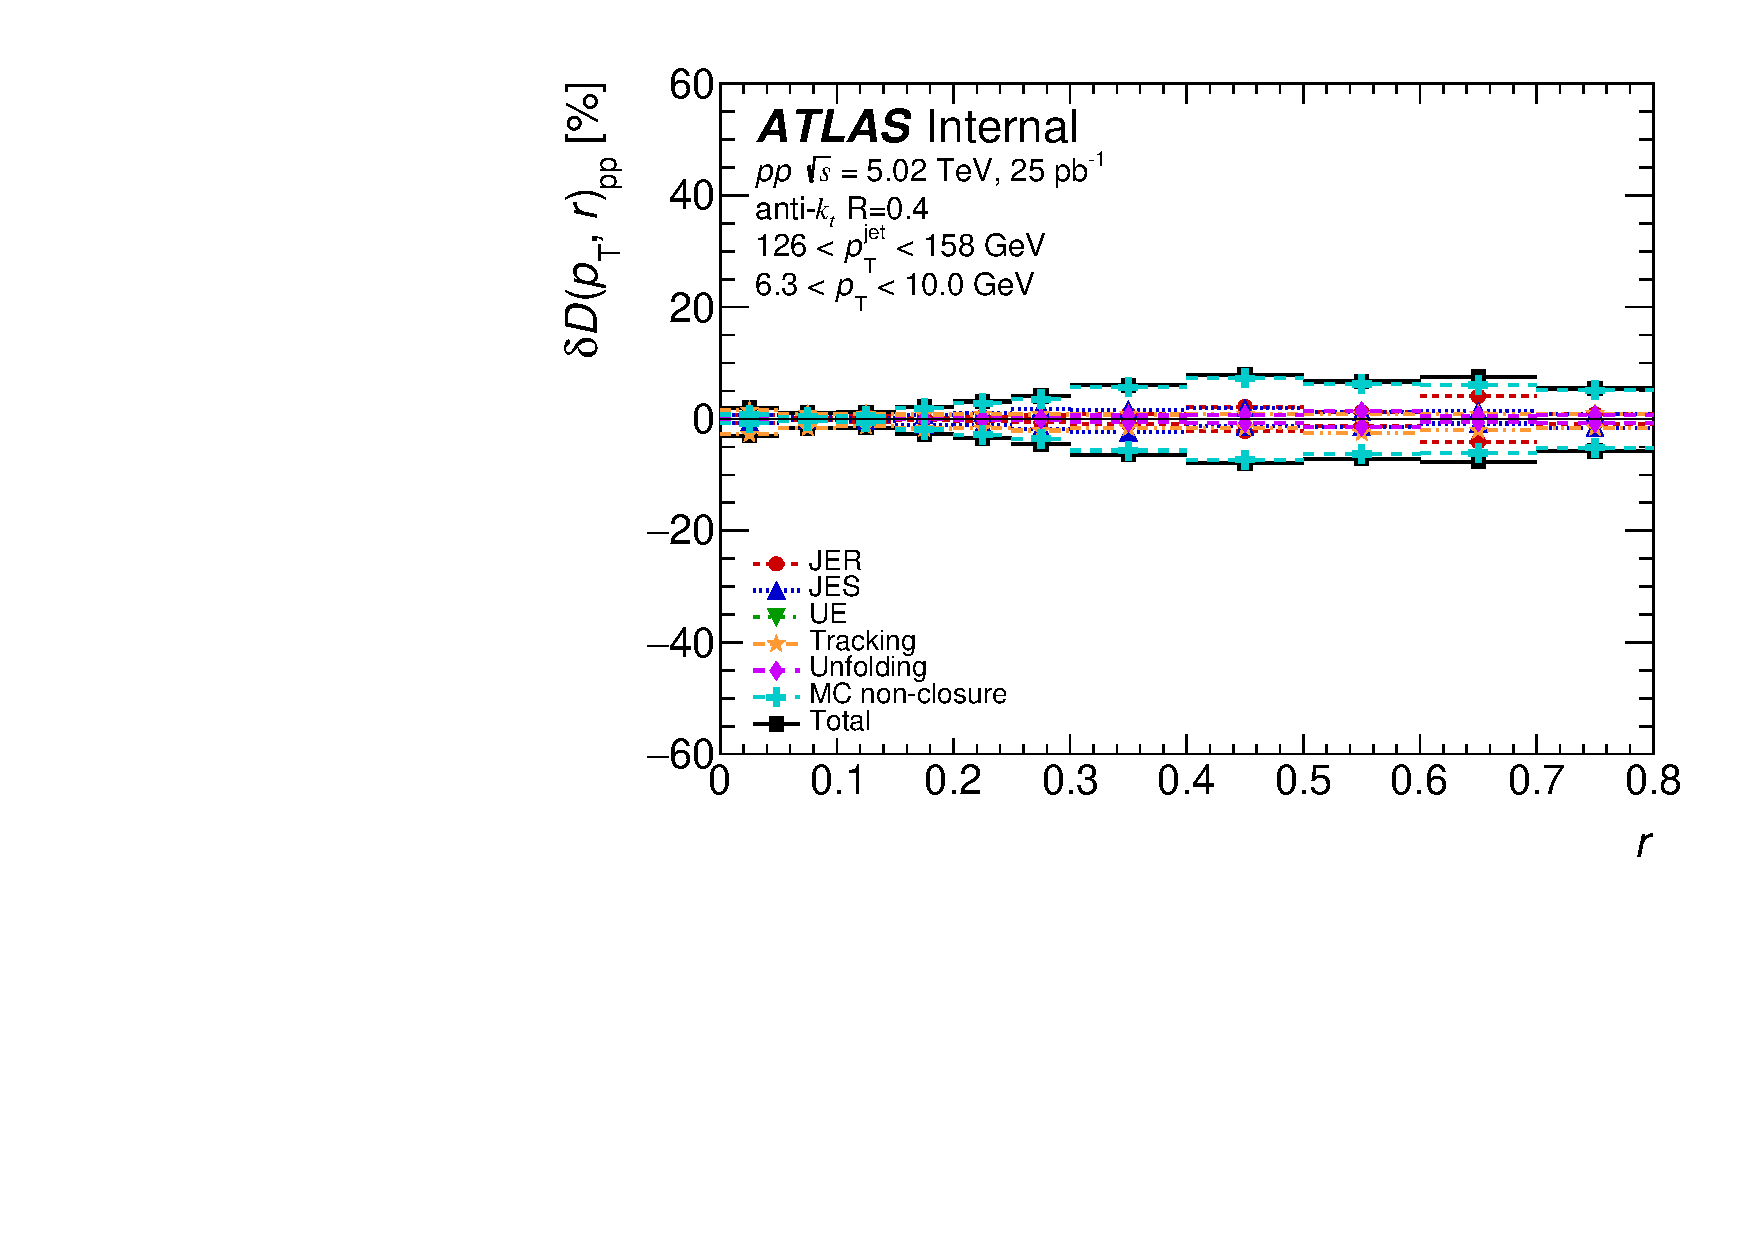
\includegraphics[width=0.53\textwidth]{figures/systematics/ChPS_dR_sys_pp_error_trk6_jet7_cent6} \\
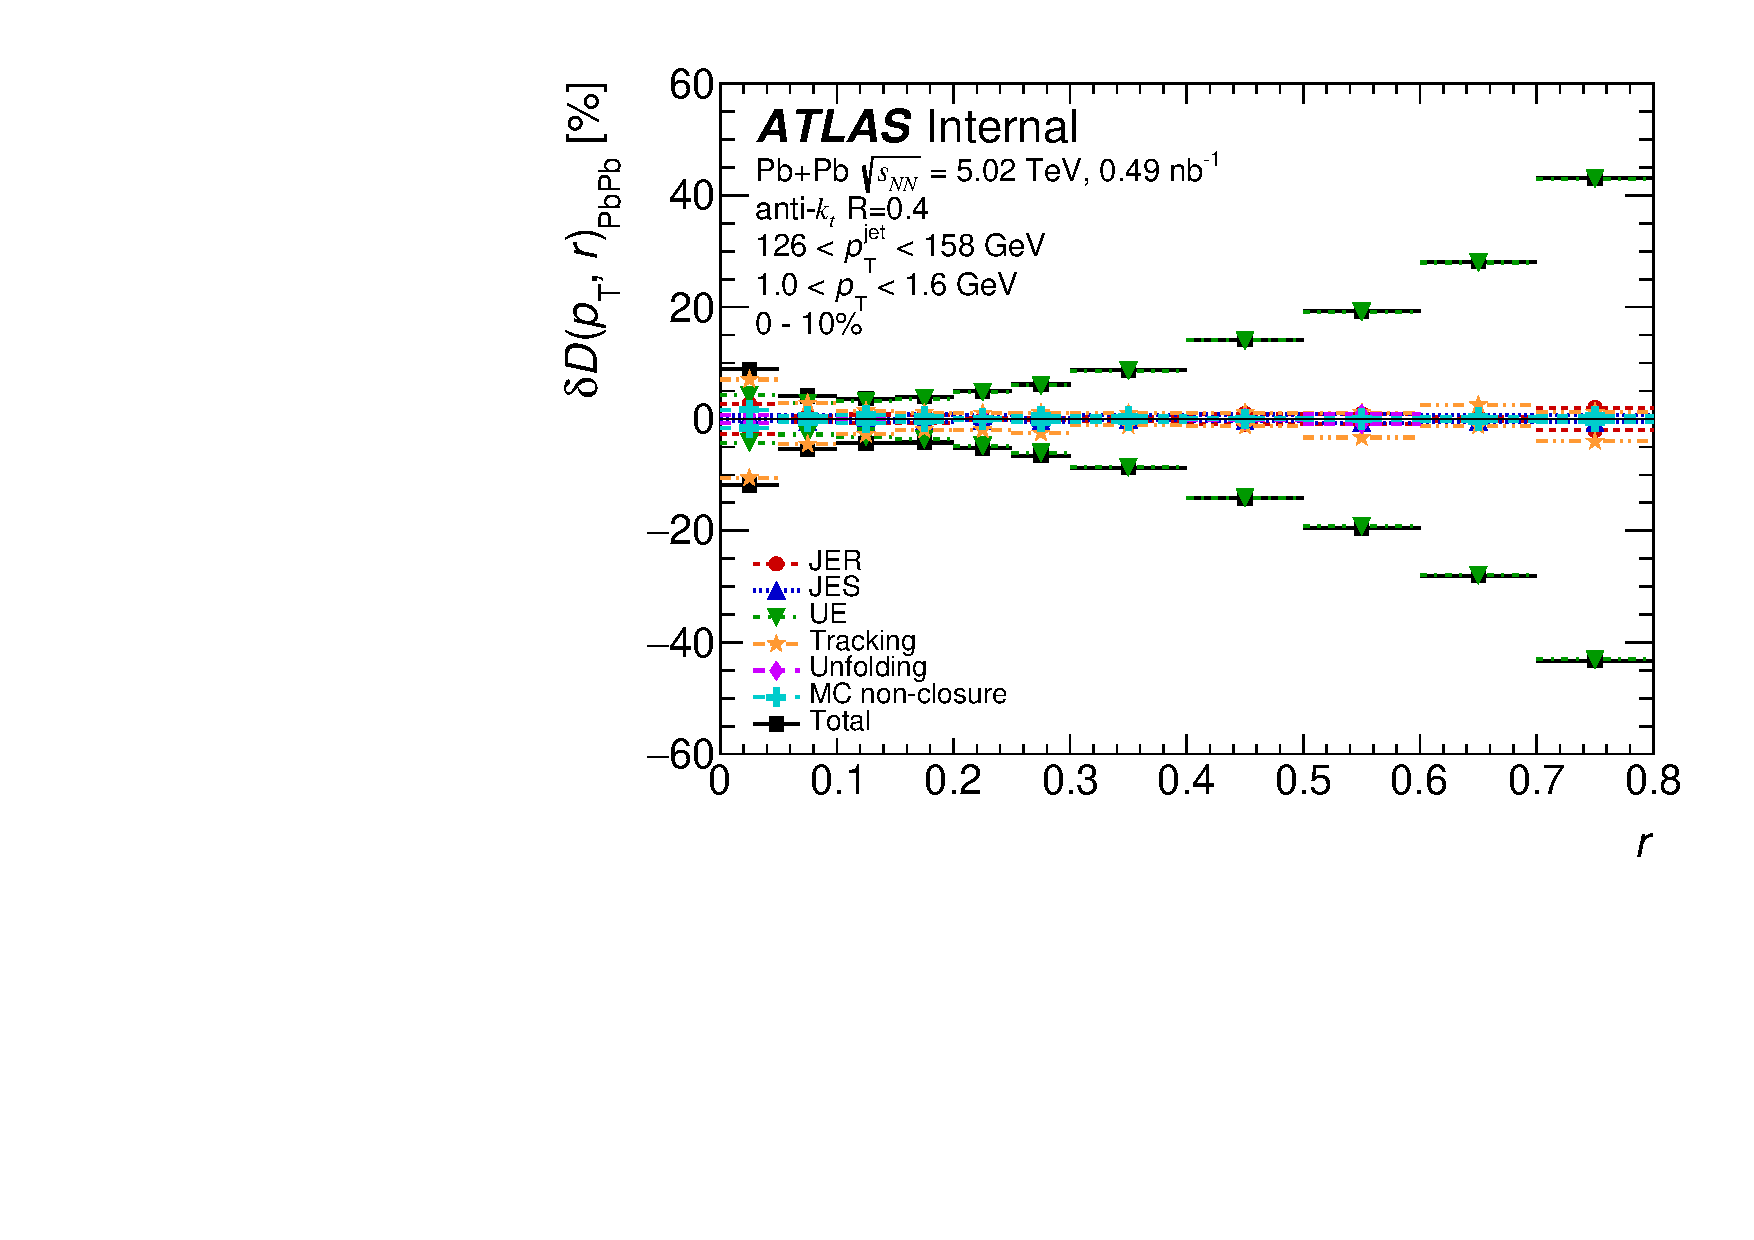
\includegraphics[width=0.53\textwidth]{figures/systematics/ChPS_dR_sys_PbPb_error_trk2_jet7_cent0} &
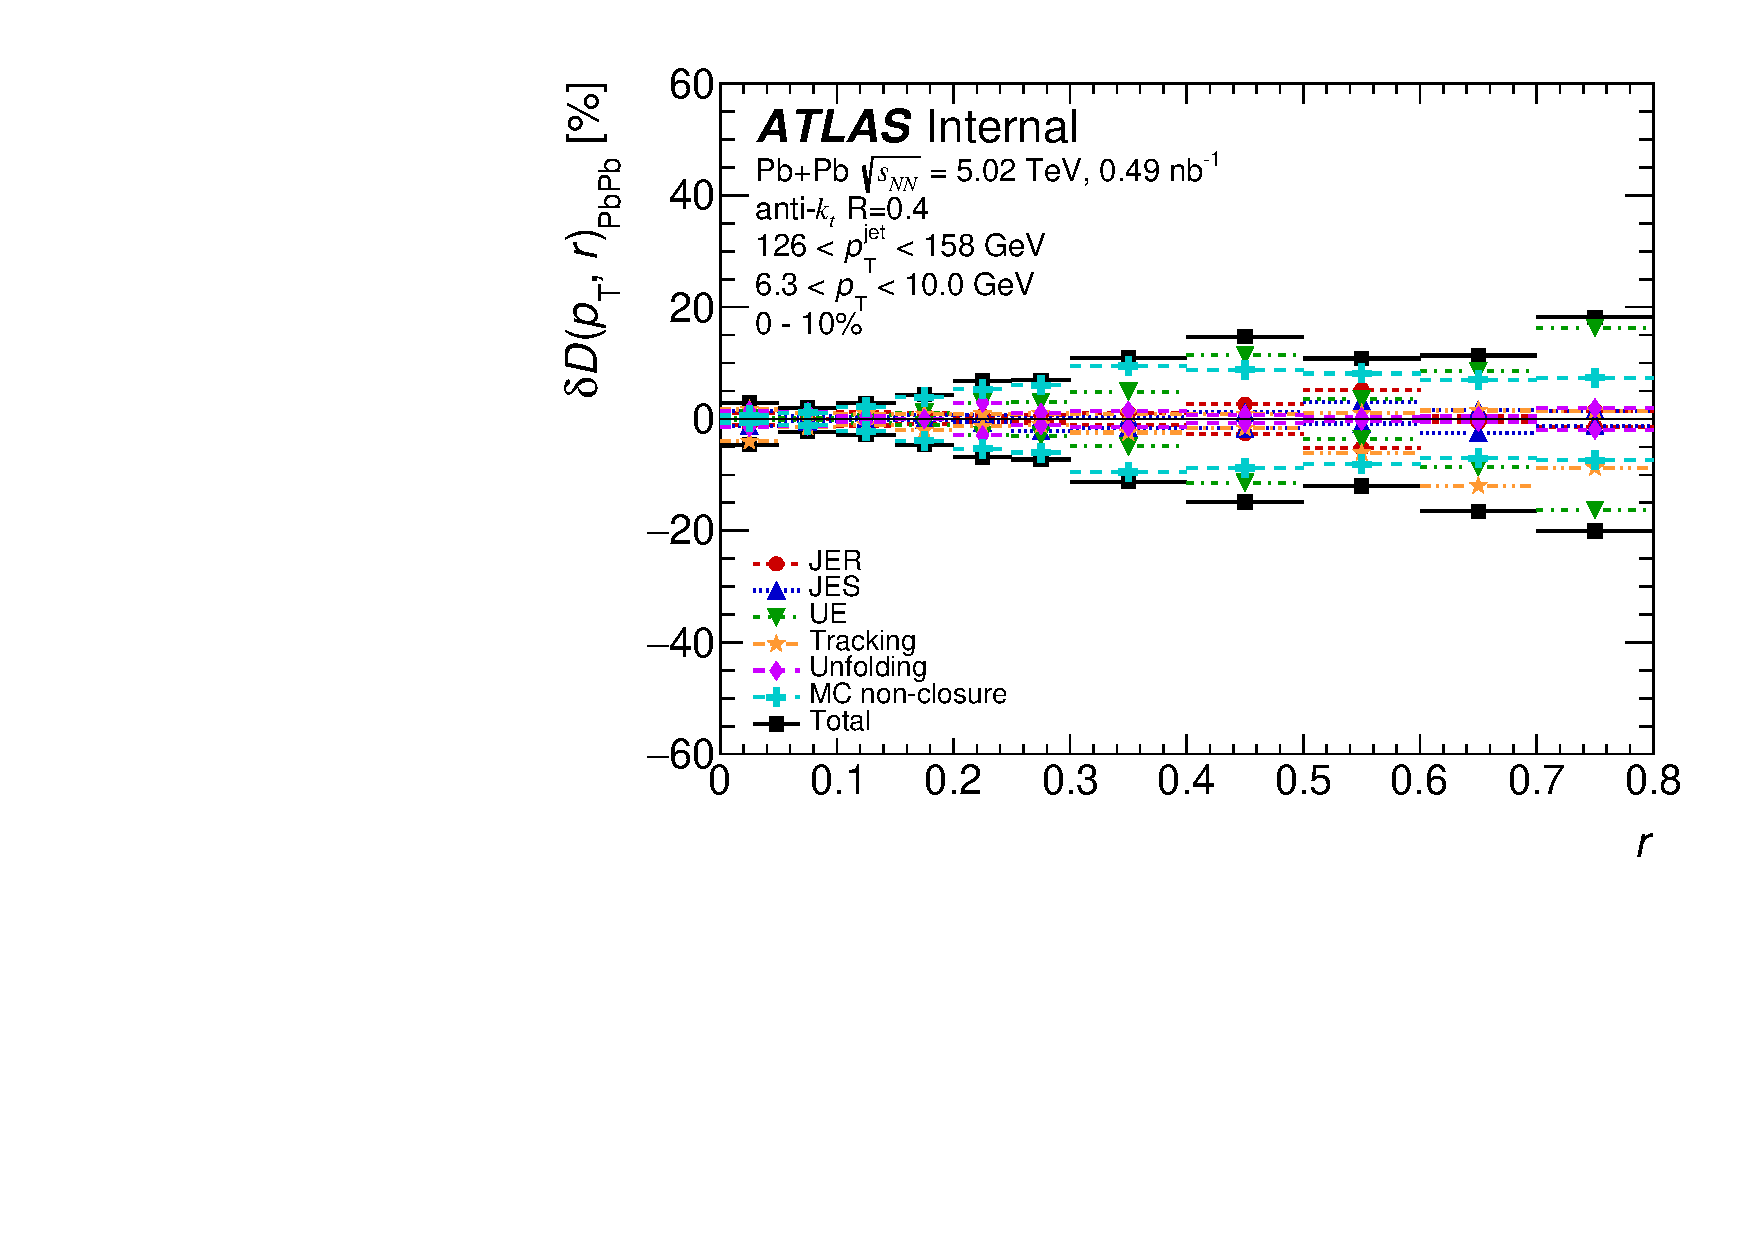
\includegraphics[width=0.53\textwidth]{figures/systematics/ChPS_dR_sys_PbPb_error_trk6_jet7_cent0} \\
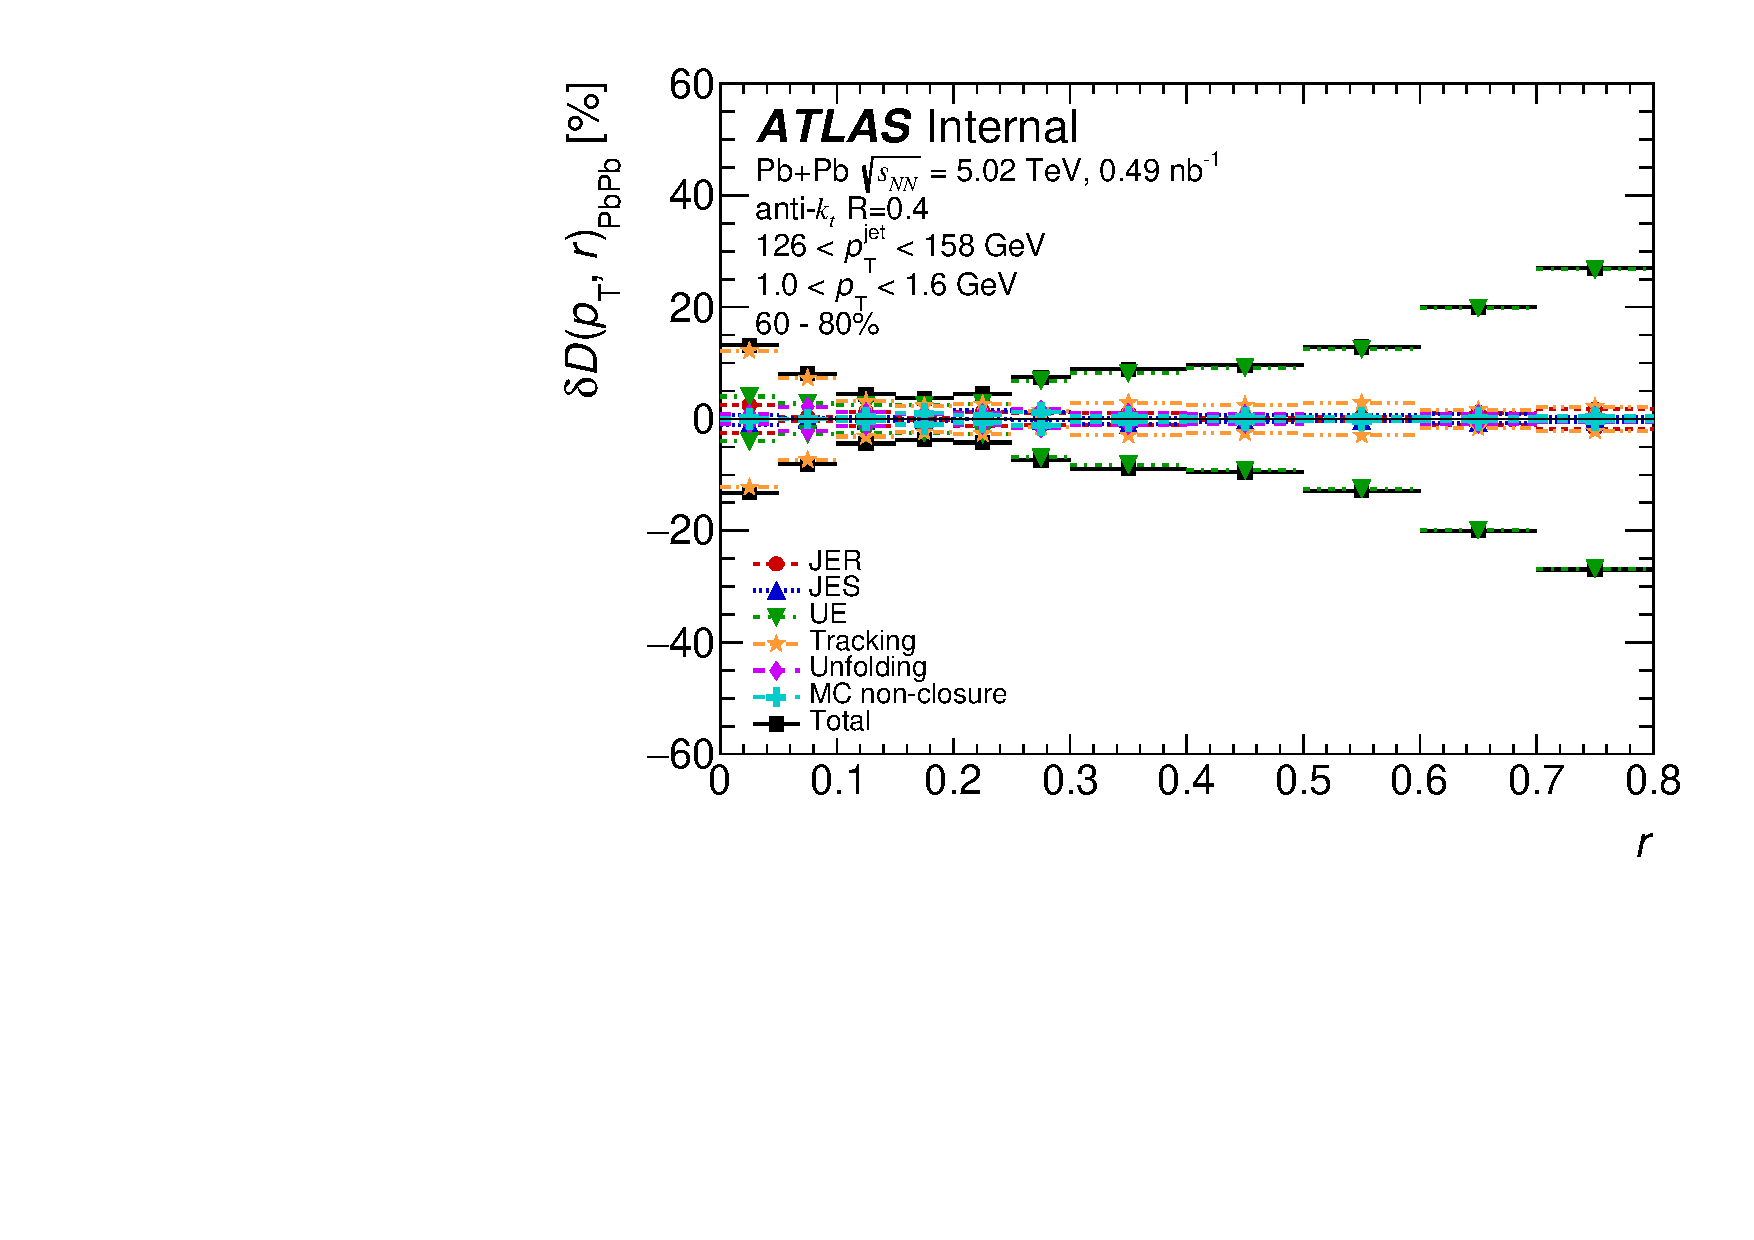
\includegraphics[width=0.53\textwidth]{figures/systematics/ChPS_dR_sys_PbPb_error_trk2_jet7_cent5} &
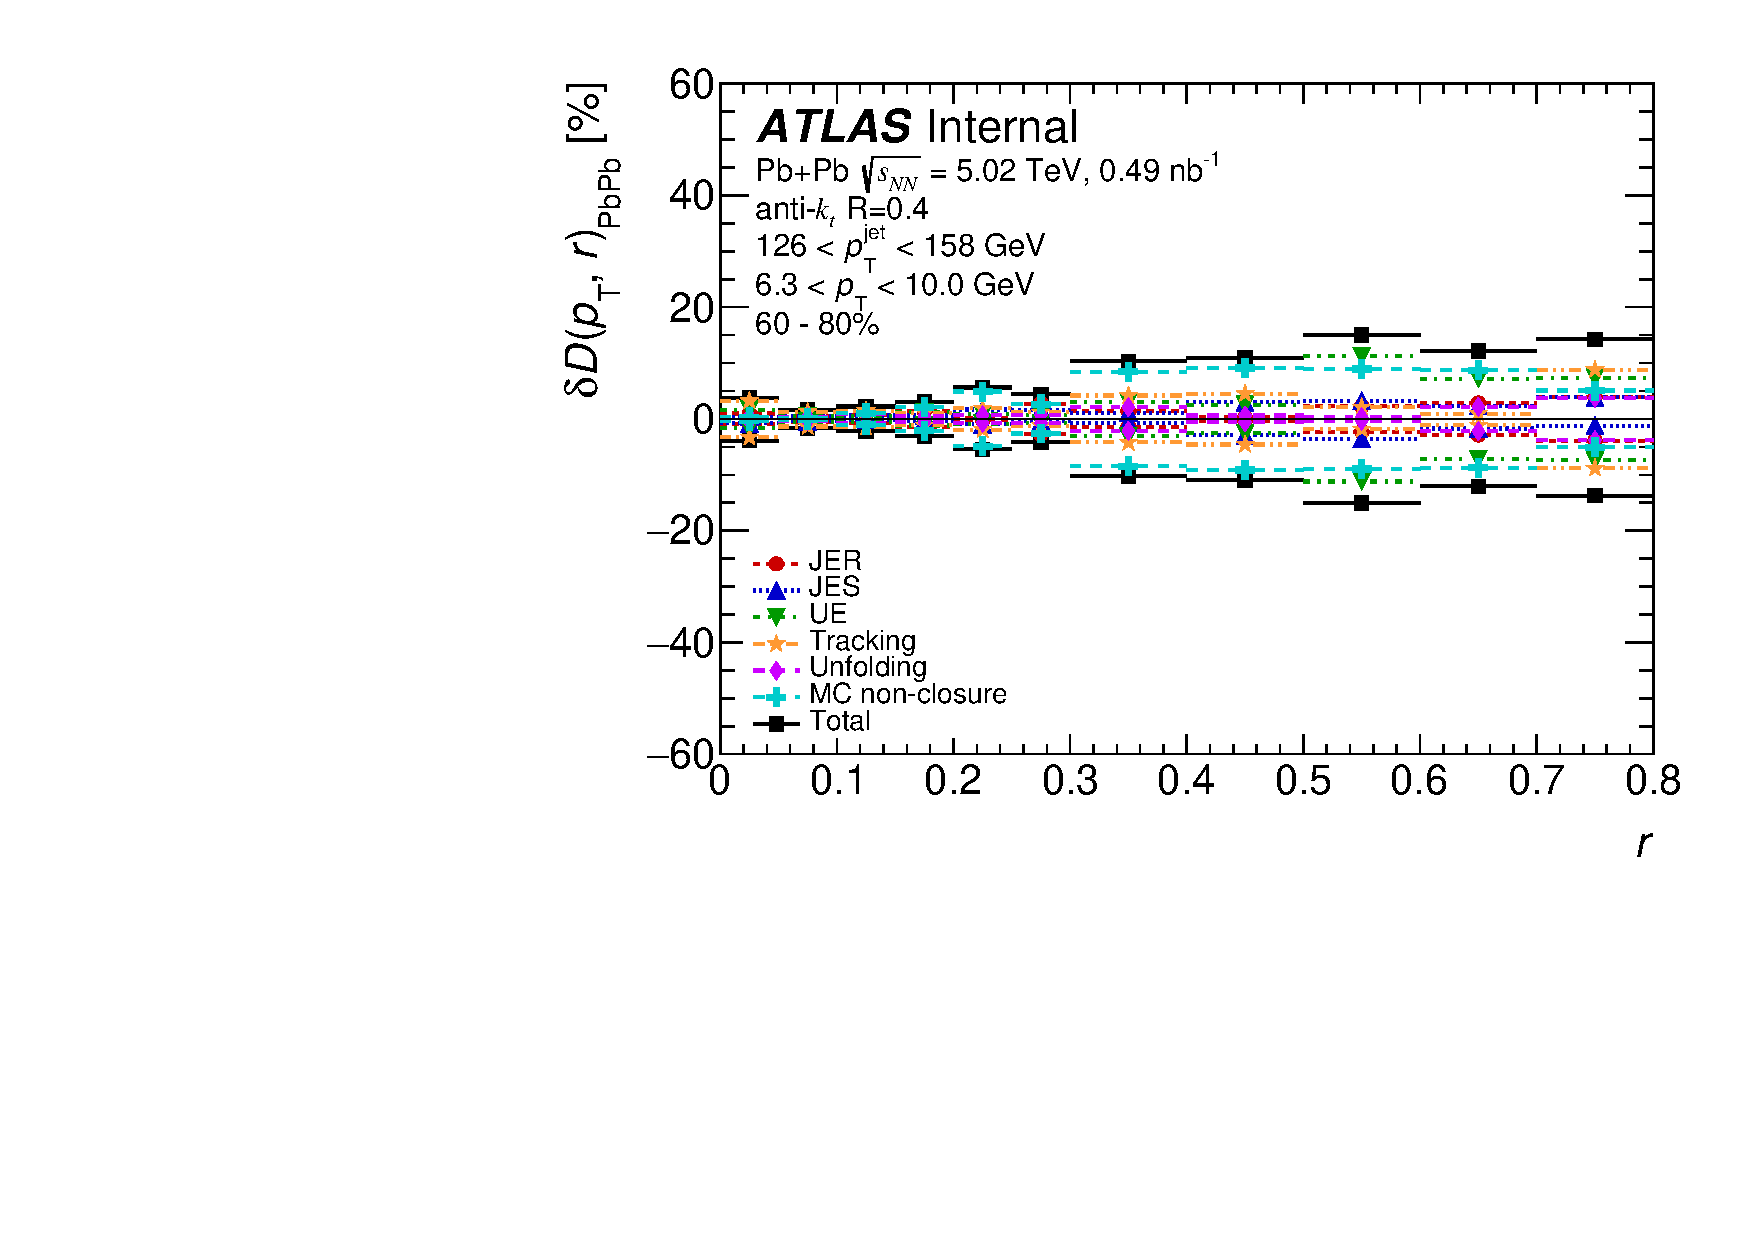
\includegraphics[width=0.53\textwidth]{figures/systematics/ChPS_dR_sys_PbPb_error_trk6_jet7_cent5} \\
\end{tabular}}
\caption{
Relative size of the systematic uncertainties for \Dptr\ distributions in \pp\ (top), central 0--10\% \pbpb\ (middle), and peripheral 60--80\% \pbpb\ (bottom) collisions for tracks with $1.0 < \pt < 1.6$ \GeV\ (left) and $6.3 < \pt < 10$ \GeV\ (right) in jets with $126 < \ptjet < 158$ \GeV. The systematic uncertainties due to JES, JER, unfolding, UE contribution, MC non-closure, and tracking are shown along with the total systematic uncertainty from all sources.
}
\label{fig:Systematics_Dpt}
\end{figure}

\begin{figure}
\centerline{
\begin{tabular}{cc}
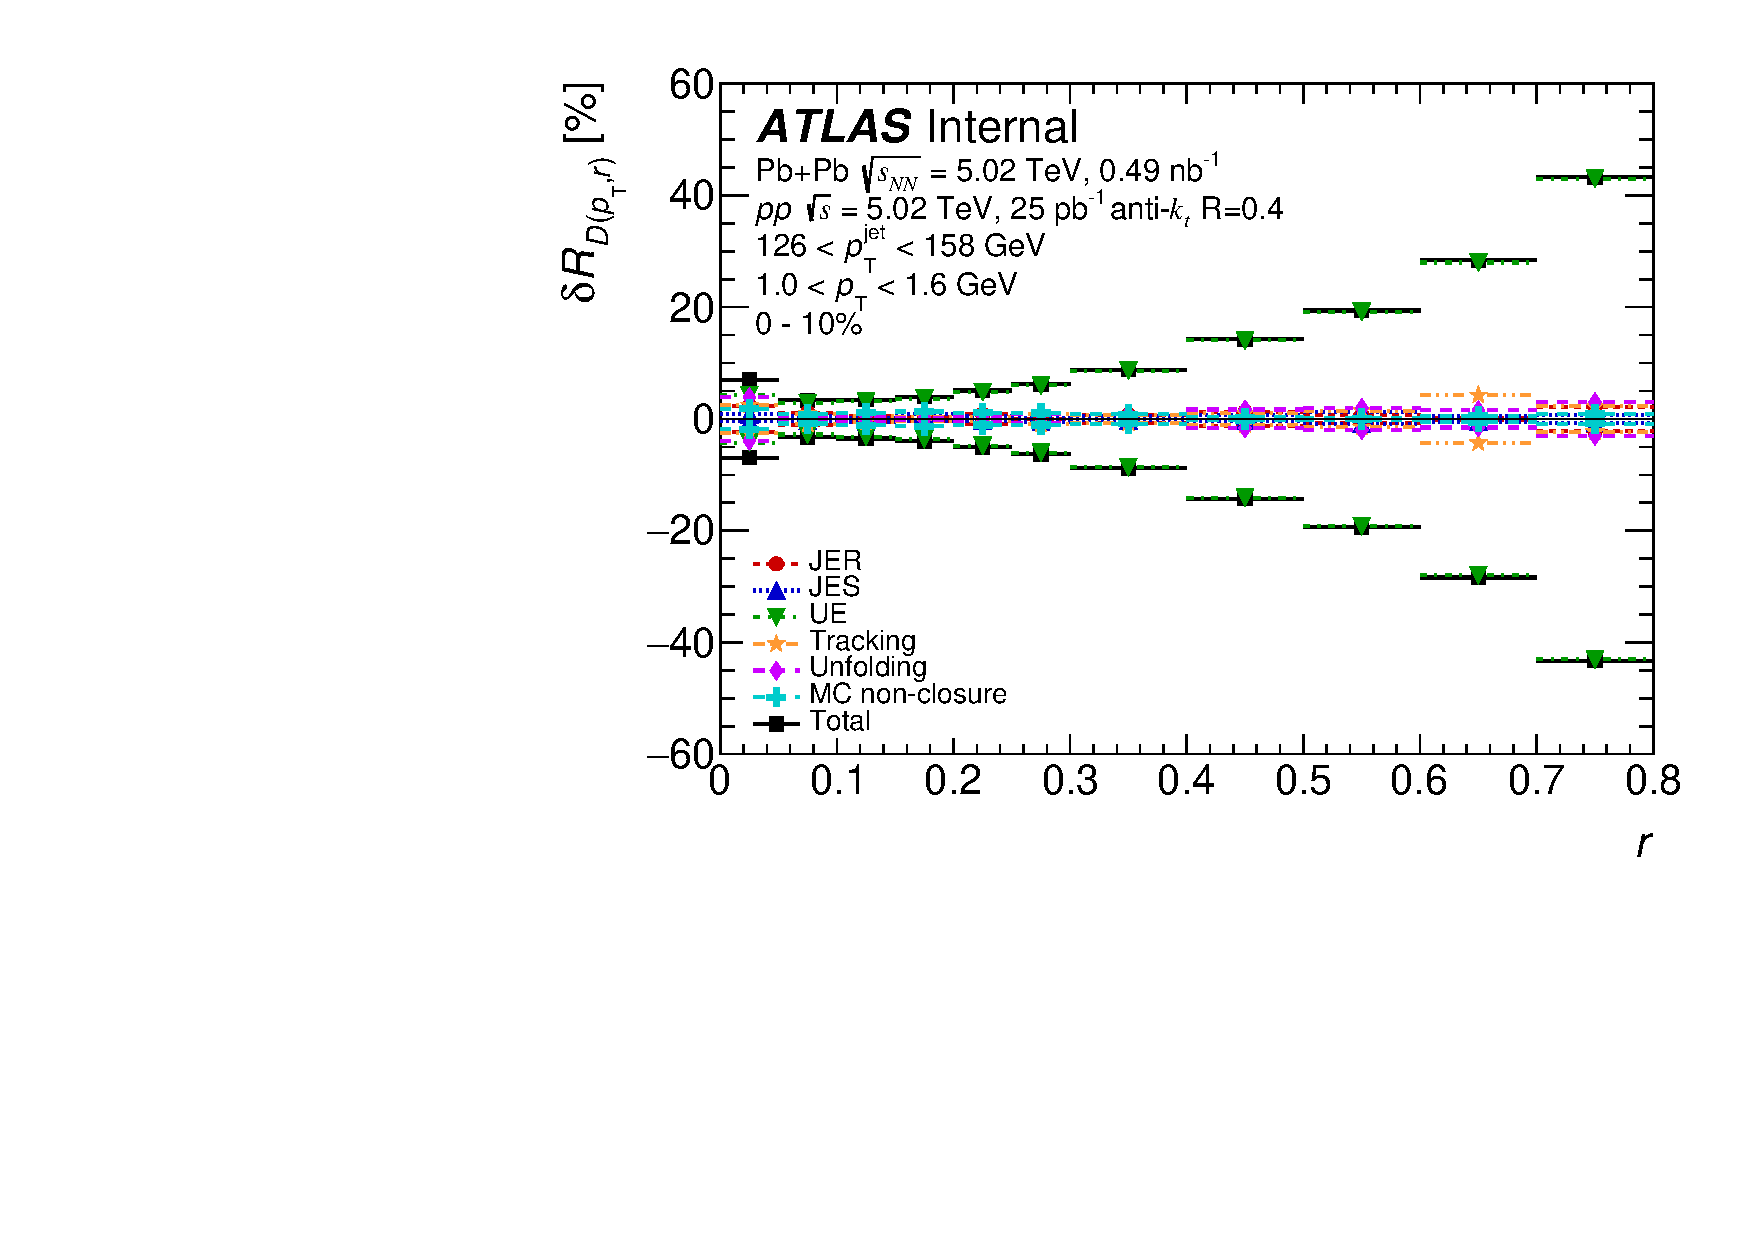
\includegraphics[width=0.53\textwidth]{figures/systematics/RDpT_dR_sys_error_trk2_jet7_cent0} &
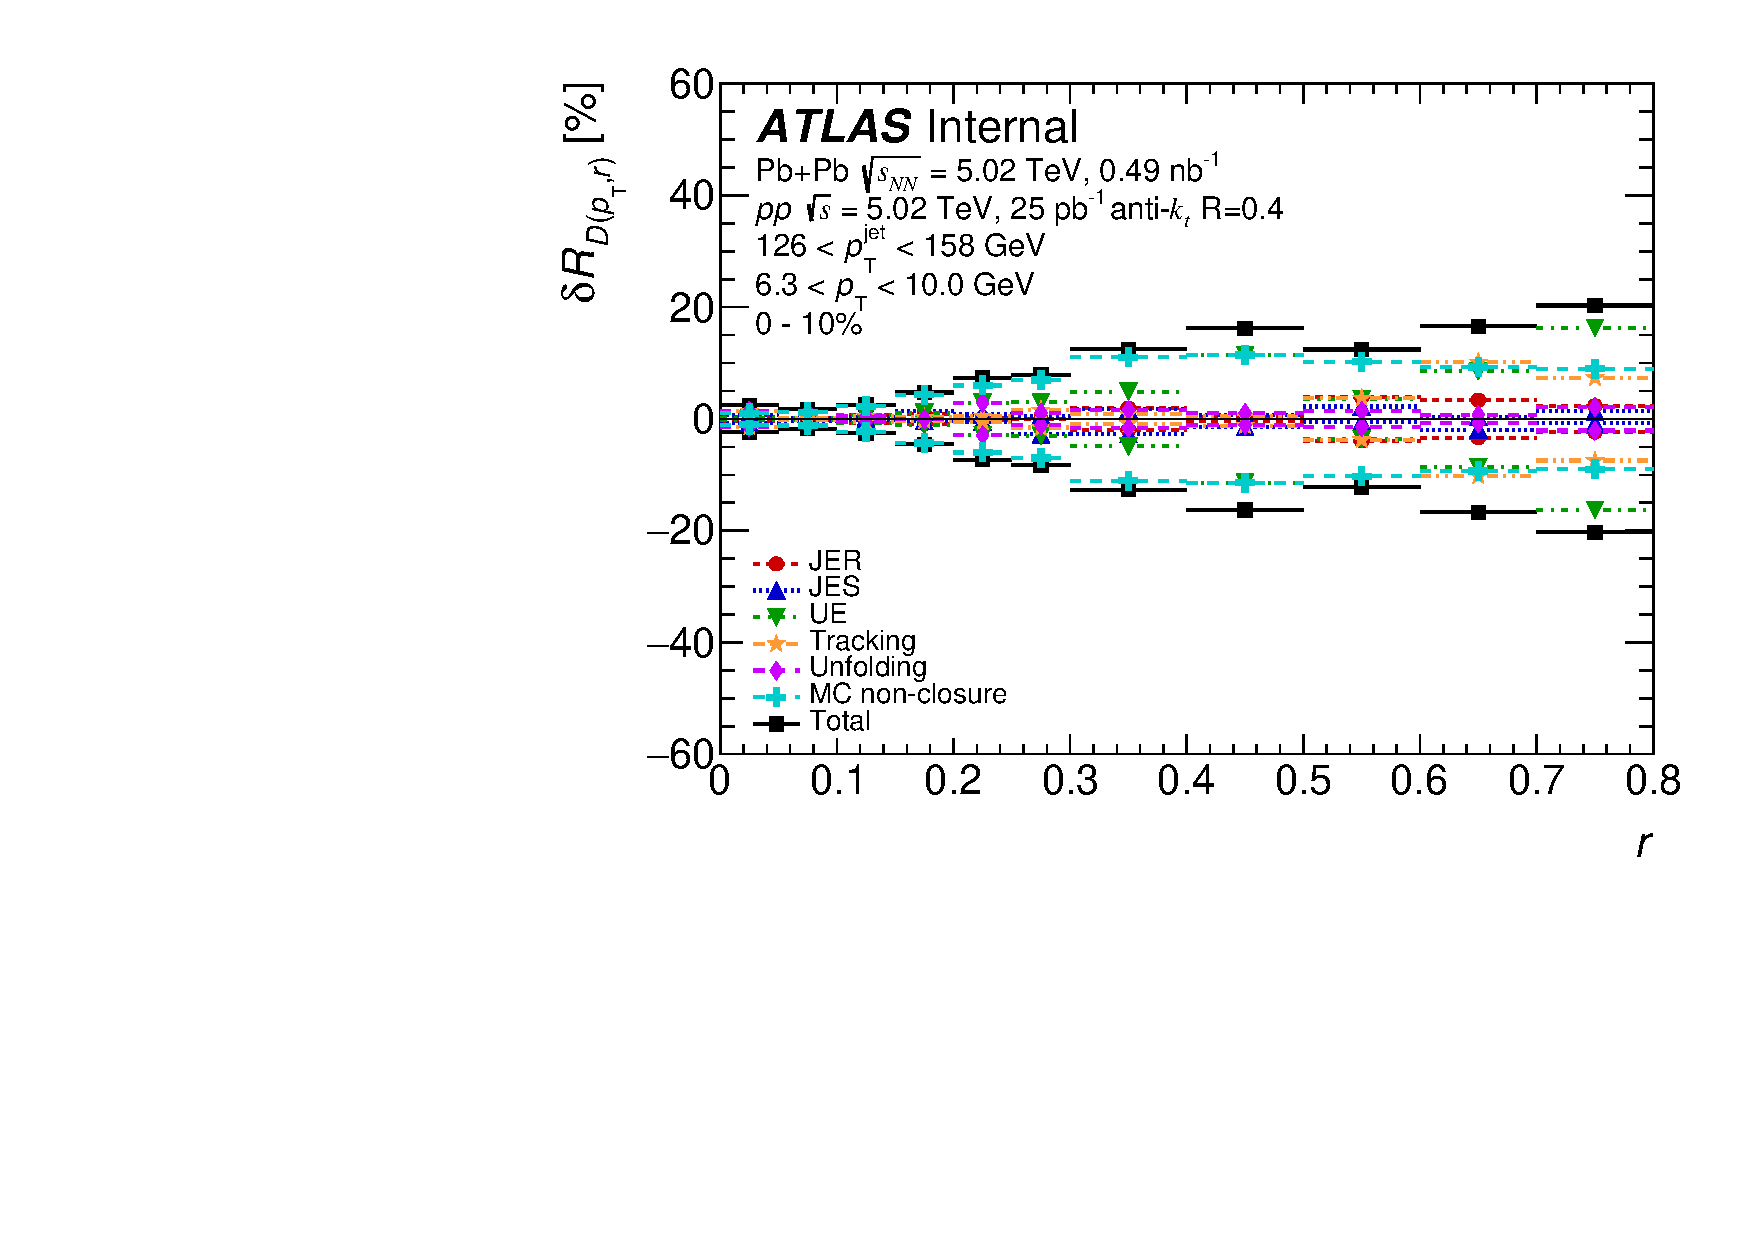
\includegraphics[width=0.53\textwidth]{figures/systematics/RDpT_dR_sys_error_trk6_jet7_cent0} \\
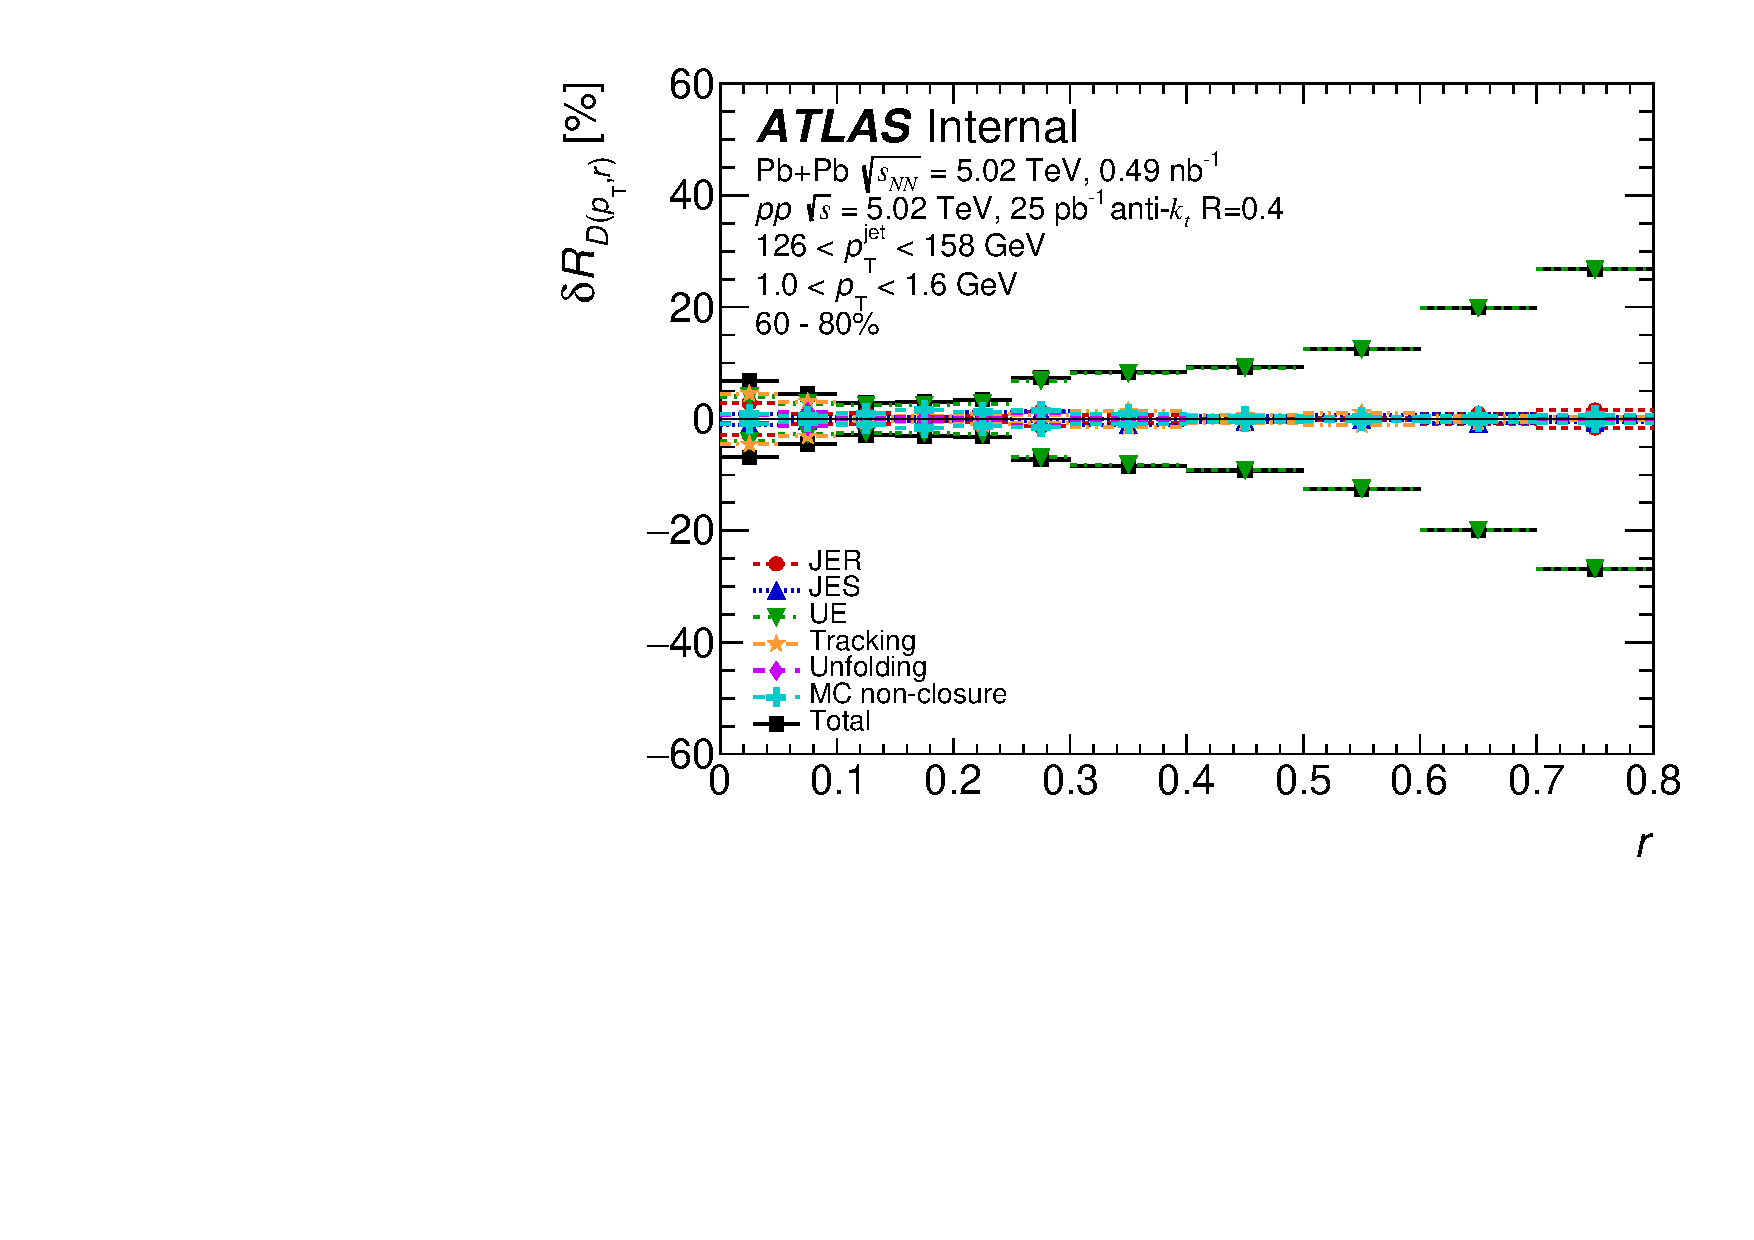
\includegraphics[width=0.53\textwidth]{figures/systematics/RDpT_dR_sys_error_trk2_jet7_cent5} &
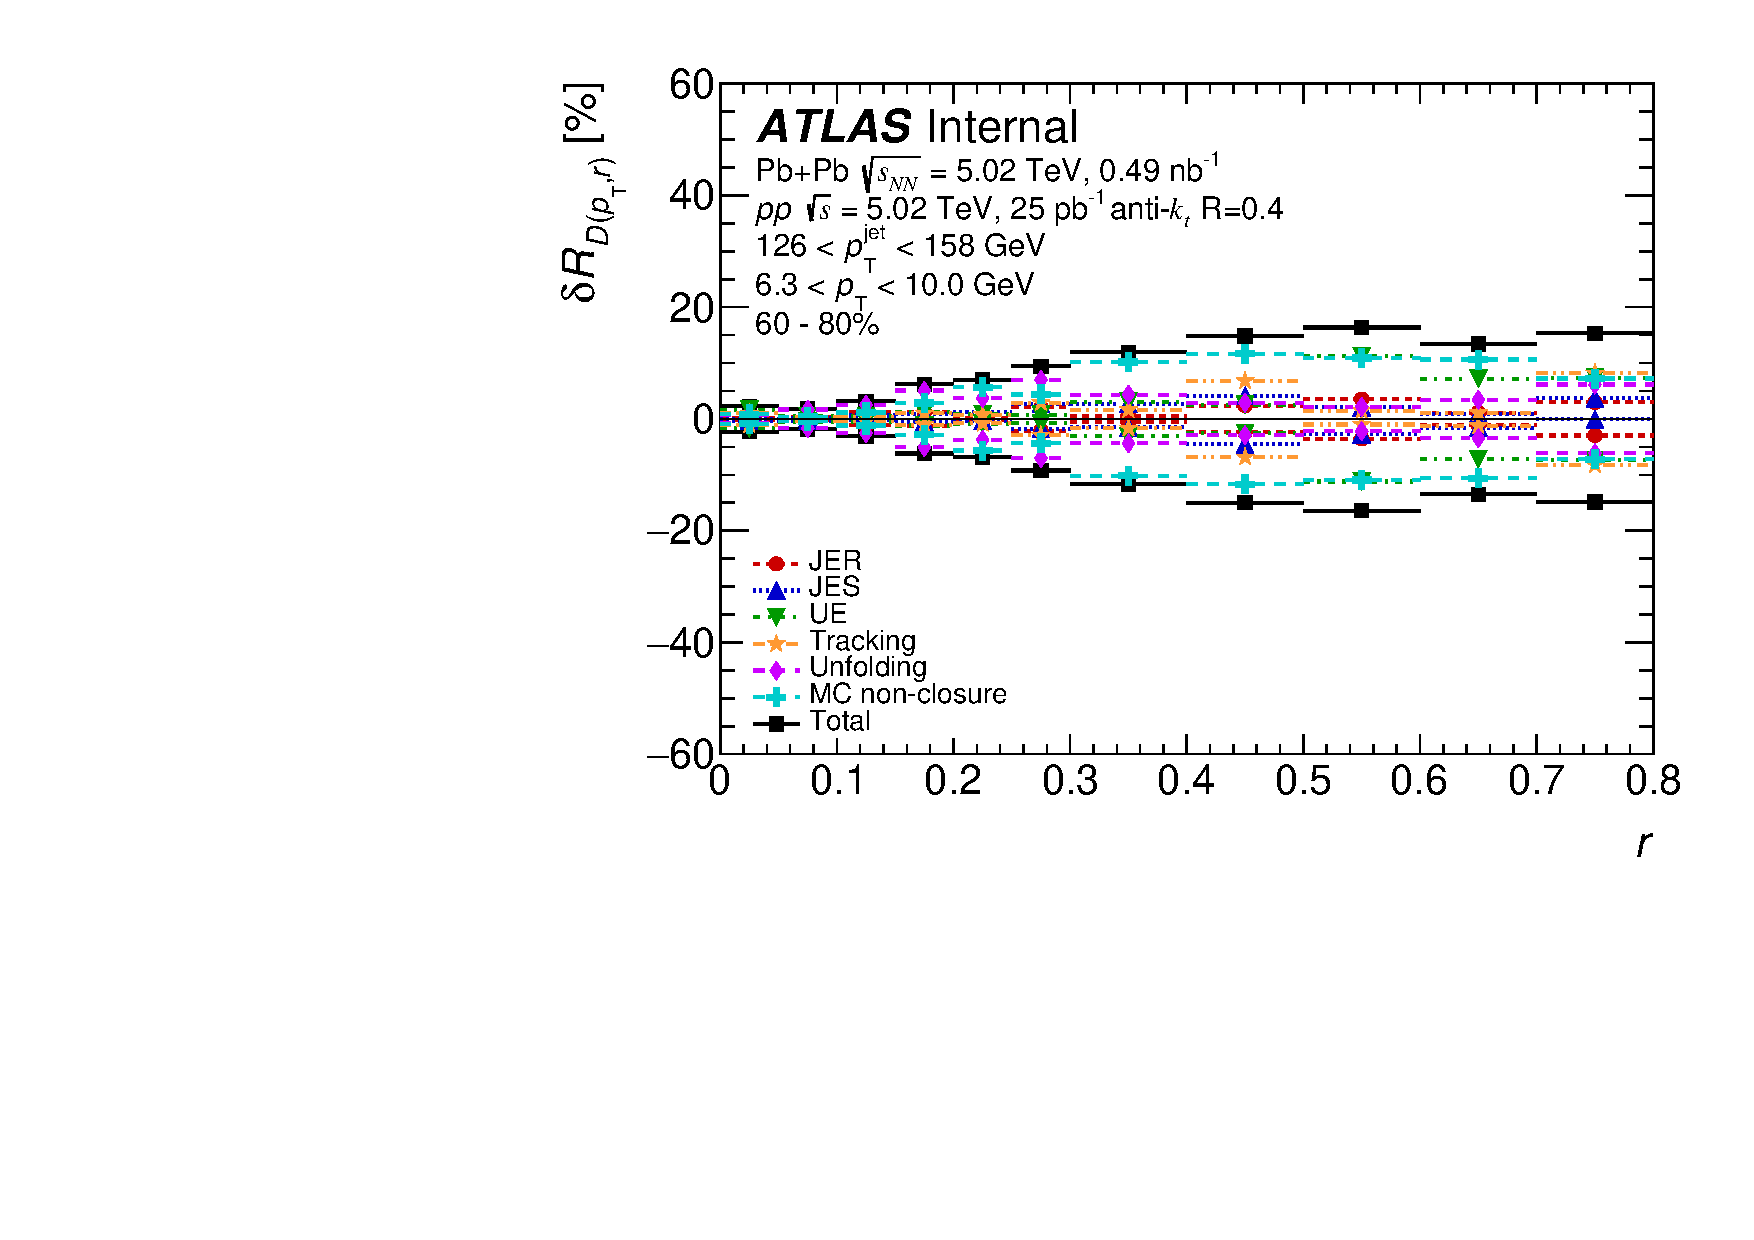
\includegraphics[width=0.53\textwidth]{figures/systematics/RDpT_dR_sys_error_trk6_jet7_cent5} \\
\end{tabular}}
\caption{
Relative size of the systematic uncertainties for \RDptr\ distributions for 0--10\% (top) and 60--80\% (bottom) \pbpb\ collisions, for tracks with $1.0 < \pt < 1.6$ \GeV\ (left) and $6.3 < \pt < 10.0$ \GeV\ (right), in jets with $126 < \ptjet < 158$ \GeV. The systematic uncertainties due to JES, JER, unfolding, UE contribution, MC non-closure, and tracking are shown along with the total systematic uncertainty from all sources.
}
\label{fig:Systematics_RDpT}
\end{figure}

%\begin{figure}
%\centerline{
%\begin{tabular}{cc}
%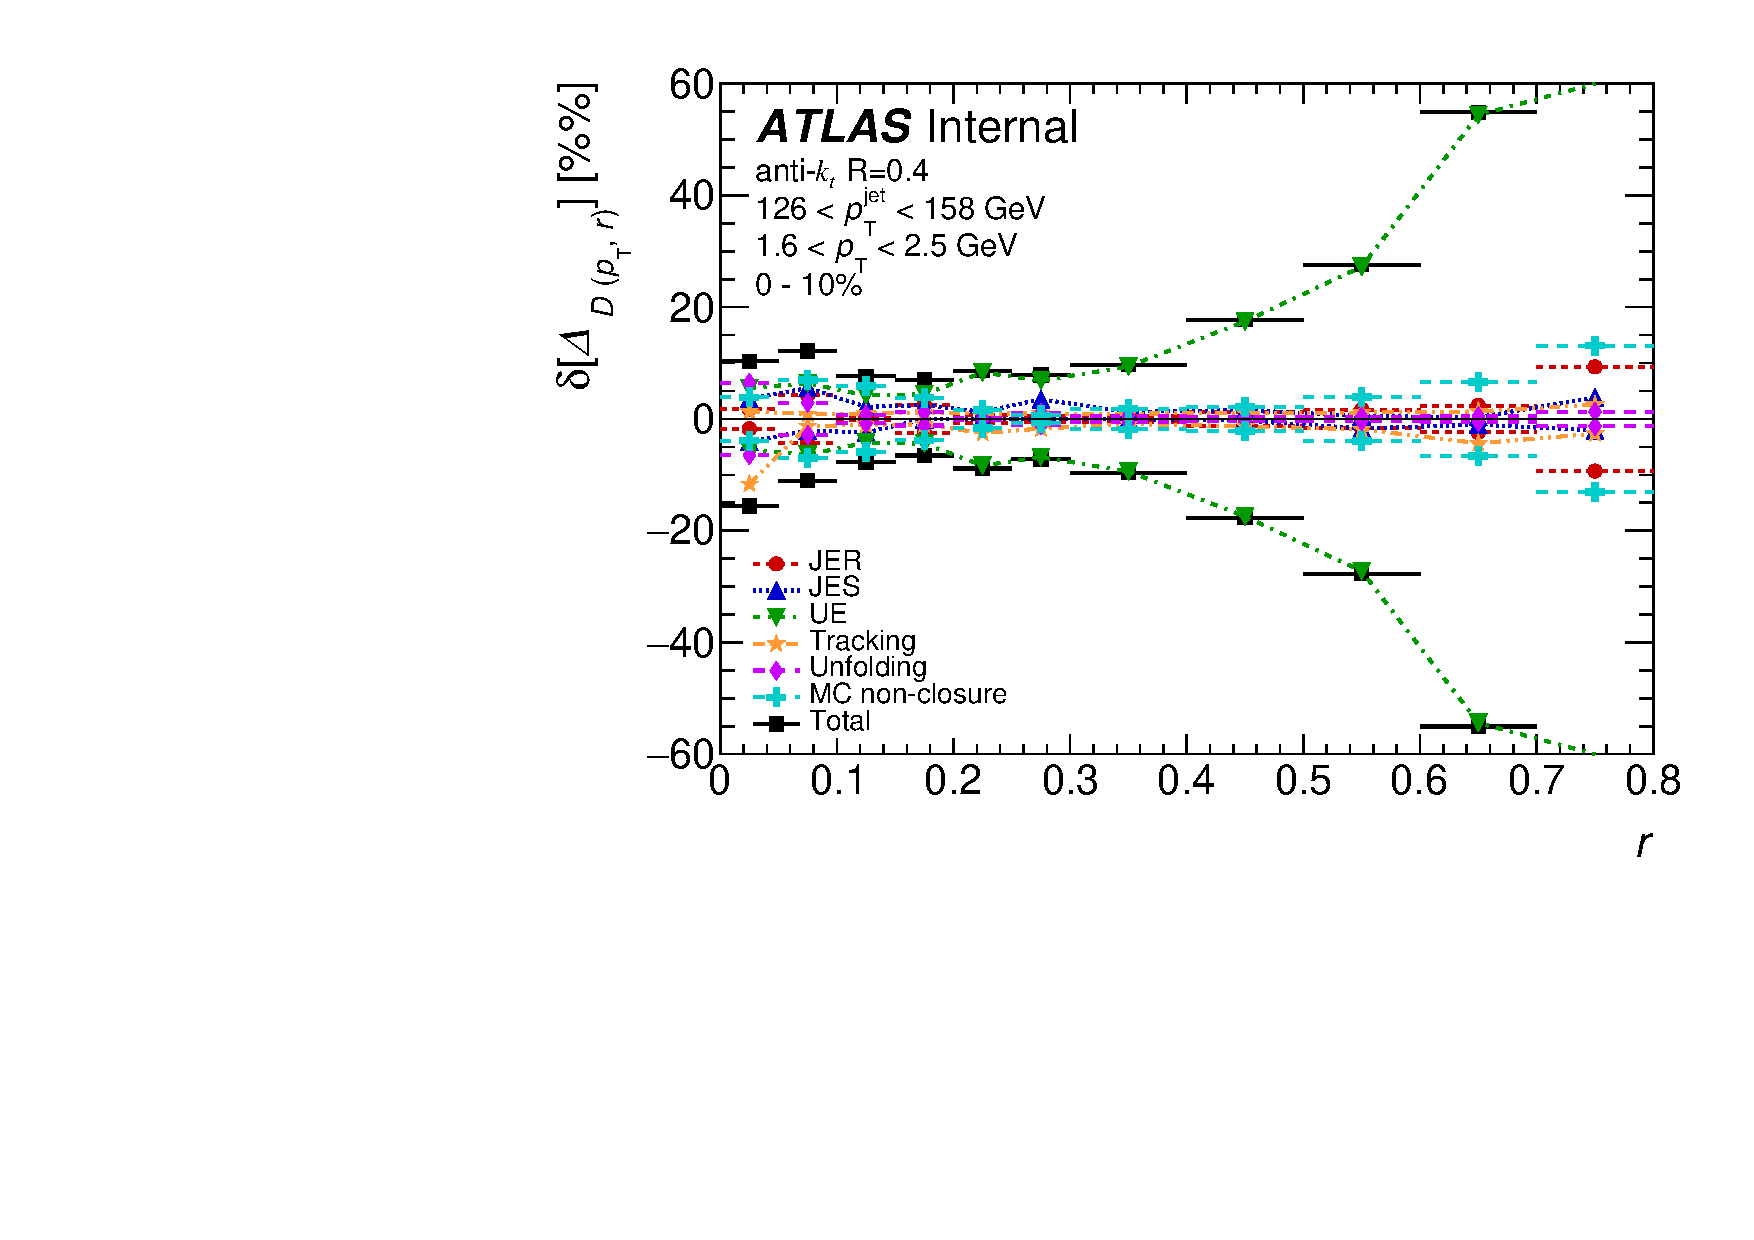
\includegraphics[width=0.55\textwidth]{figures/systematics/DeltaDpT_dR_sys_error_trk3_jet7_cent0} &
%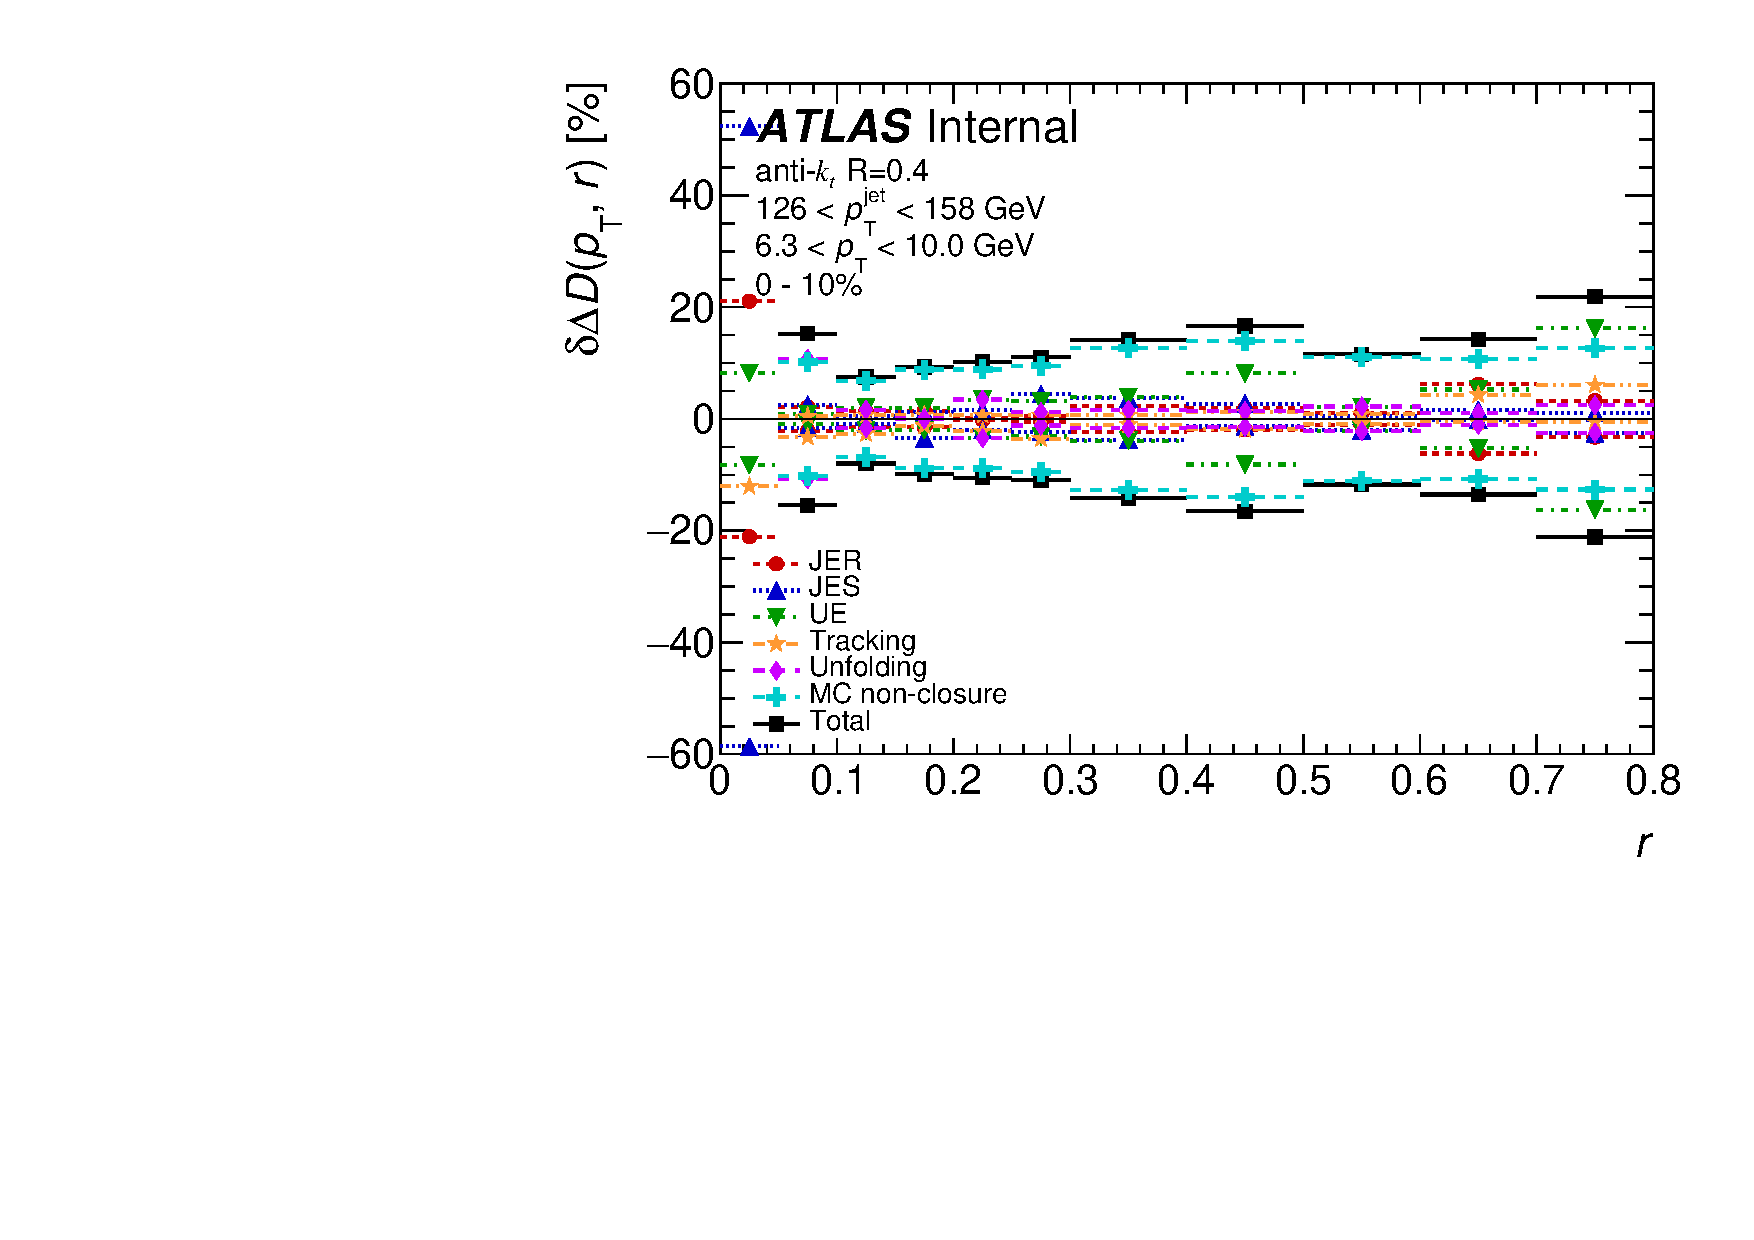
\includegraphics[width=0.55\textwidth]{figures/systematics/DeltaDpT_dR_sys_error_trk6_jet7_cent0} \\
%\end{tabular}}
%\caption{
%Relative size of the systematic uncertainties for $\Delta\Dptr$ distributions for 0--10\% \pbpb\ collisions, for tracks in the \pt\ range 1.0--1.6 \GeV\ (left) and 6.3--10.0 \GeV\ (right), in jets with $126 < \ptjet < 158$ \GeV. The systematic uncertainties due to JES, JER, unfolding, UE contribution, MC non-closure and tracking are shown along with the total systematic uncertainty from all sources.
%}
%\label{fig:Systematics_DeltaDpT}
%\end{figure}

